\documentclass{article}
\usepackage{graphicx} % Required for inserting images
\graphicspath{ {./Images/} }
\usepackage{pdfpages}
\newcommand{\insertslide}[2]{%
\hspace*{-2.4cm}
\fbox{\includegraphics[page=#2,scale=0.5]{#1}}
}
% \insertslide{Slides/CM1.pdf}{1} to insert first page of CM1.pdf, for example.
\usepackage{amsmath}
\renewcommand{\familydefault}{\sfdefault}

\title{Synthèse LINFO1252}
\author{Quentin Bodart}
\date{Q1 2024-2025}

\begin{document}
\maketitle
\tableofcontents
\pagebreak

\section*{Objectifs du cours}
    \begin{itemize}
        \item utiliser et comprendre les systèmes informatiques (i.p. GNU/Linux)
        \item utiliser les services fournis par les SE (systèmes d'exploitation)
        \item design et mise en oeuvre d'un SE
    \end{itemize}

\section{CM 1}
    \subsection{Le système informatique et le rôle du système d’exploitation}
    \textbf{Syllabus} : https://sites.uclouvain.be/SystInfo/notes/Theorie/intro.html

        \subsubsection{Fondamentaux}
            \begin{itemize}
                \item Composants :
                \begin{itemize}
                    \item CPU / Processeur
                    \item Mémoire Principale (RAM)
                    \item Dispositifs d’entrée/sortie (y.c. de stockage)
                \end{itemize}
                \item Fonctionnement d'un CPU
                \begin{itemize}
                    \item Lire / écrire en mémoire vers / depuis des registres
                    \item Opérations (calculs, comparaisons) sur ces registres
                \end{itemize}
                \item Jeux d'instructions
                \begin{itemize}
                    \item x86\_64 (PC, anciens Mac)
                    \item ARM A64 (Raspberry PI, iPhone, nouveaux Mac M1–3)
                \end{itemize}
            \end{itemize}
        
        \subsubsection{Architecture de von Neumann}
            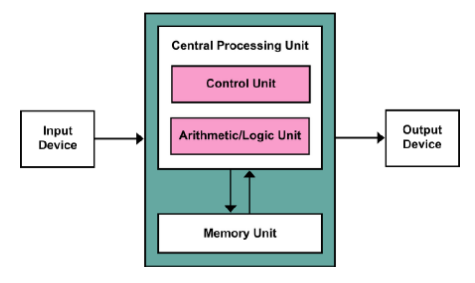
\includegraphics[scale = .5]{von_neumann.png}
        
        \subsubsection{Fonctionnement d'un système informatique}
            \begin{itemize}
                \item La représentation des données se fait en \textbf{binaire}.
                \item Les opérations d'entrée-sortie se déroule de manière concurrente.
                \item Il y existe des contrôleurs distinct controlant chacun un type de périphérique.
                \item Chaque contrôleur possède une mémoire dédiée (buffer)
                \item Le processeur doit déplacer des donnés depuis/vers la
                mémoire principale depuis/vers ces buffers dédiés
                \item Le processeur suit un "fil" continu d’instructions
                \item Le contrôleur de périphérique annonce au
                processeur la fin d’une opération d’entrée/sortie en
                générant une interruption (signal électrique à destination du processeur)
            \end{itemize}

        \subsubsection{Traitement d'une interruption}
            Le processeur interrompt le fil d’exécution d’instructions courant et
            transfert le contrôle du processeur à une routine de traitement.
            Cette même routine détermine la source de l'interruption, puis restaure l'état du processeur
            et reprend le processus :\\
            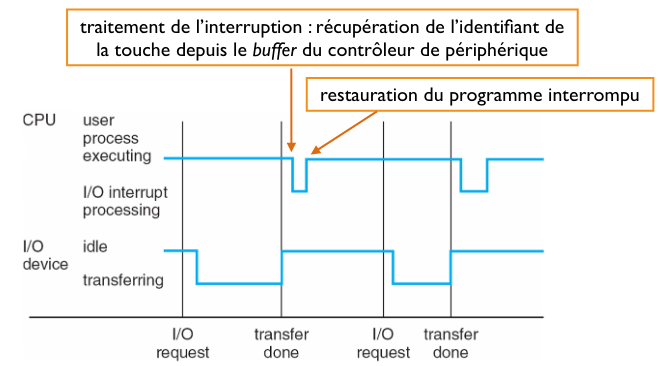
\includegraphics[scale=.75]{interruption.png}

        \subsubsection{Accès direct à la mémoire}
            Direct Memory Access (DMA) désigne le fait de ne pas faire une interruption à chaque octet lu depuis un disque dur.
            Une interruption est tout de même faite à la fin du transfert d'un \textbf{bloc}.
        
        \subsubsection{Système informatique complet}
            \includegraphics*[scale=.85]{systeme_complet.png}
        
        \subsubsection{Rôle du système d'exploitation}
            Programmer directement au-dessus du matériel, gérer les interruption, etc... serait une trop grosse tâche pour le programmeur.\\\\
            3 rôles principaux
            \begin{itemize}
                \item Rendre l’utilisation et le développement d’applications
                plus simple et plus universel (portable d’une machine à
                une autre)
                \item Permettre une utilisation plus efficace des ressources
                \item Assurer l’intégrité des données et des programmes
                entre eux (e.g., un programme crash mais pas le système)
            \end{itemize}
        
        \subsubsection{Virtualisation}
            Le système d'expoitation \textbf{virtualise} les ressources matérielles afin de fonctionner de la même manière sur des systèmes avec des ressources et composants fort différents.
            Chaque SE doit trouver un compromis entre abstraction et efficacité !

        \subsubsection{Séparation entre mécanisme et politique}
            \begin{itemize}
                \item Un mécanisme permet le partage de temps
                \item Une politique arbitre entre les processus pouvant s’exécuter
                et le(s) processeur(s) disponibles
            \end{itemize}
            On peut définir des politiques d’ordonnancement différentes selon les contextes, mais sur la base du même mécanisme.
        
        \subsubsection{Modes d'exécution}
            \begin{itemize}
                \item mode utilisateur : programme utilisant les abstractions
                fournies par le SE ; certaines instructions sont interdites, comme par exemple:
                \begin{itemize}
                    \item Accès à une zone mémoire non-autorisée (SegFault)
                    \item De manière générale, toutes les instructions permettant de
                    changer la configuration matérielle du système, comme la
                    configuration ou la désactivation des interruptions
                \end{itemize}
                \item mode protégé : utilisé par le noyau du SE, toutes les
                instructions sont autorisées
                \item L’utilisation de fonctionnalités du SE par un processus
                utilisateur nécessite de passer d’un mode à l’autre : \textbf{appel système}
            \end{itemize}
        
        \subsubsection{Appel système}
            \begin{itemize}
                \item Un appel système permet à un processus utilisateur
                d’invoquer une fonctionnalité du SE
                \item Le processeur interrompt le processus, passe en mode
                protégé, et branche vers le point d’entrée unique du noyau :\\
                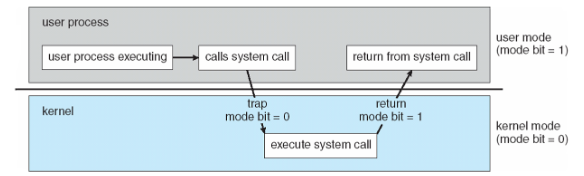
\includegraphics[scale=.75]{appel_systeme.png}
            \end{itemize}
                
            %TODO

    \subsection{Utilisation de la ligne de commande}
    \textbf{Syllabus} : https://sites.uclouvain.be/SystInfo/notes/
    Theorie/shell/shell.html

            \subsubsection{Utilitaires UNIX}
                La philosophie lors de la création des utilitaires UNIX était
                de créer des outils les plus simples possible,
                donc d'avoir une seule tâche par outil :\\
                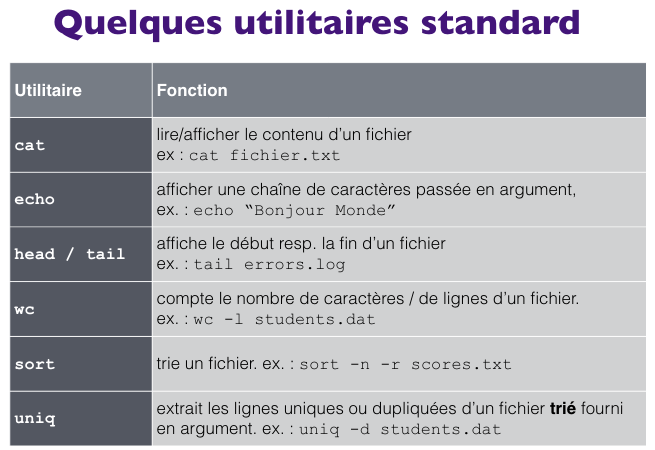
\includegraphics[scale=.5]{utilitaires_unix.png}
                Afin d'en savoir plus sur unecommande, il suffit d'utiliser l'utilitaire `man`.
            
            \subsubsection{Shell / Interpréteur de commandes}
                Rend possible l'interaction avec le SE.
                Il en existe plusieurs, mais le principal est `bash`.
                Il est toujours complémentaire à une \textbf{interface graphique}.
            
            \subsubsection{Flux et redirections}
                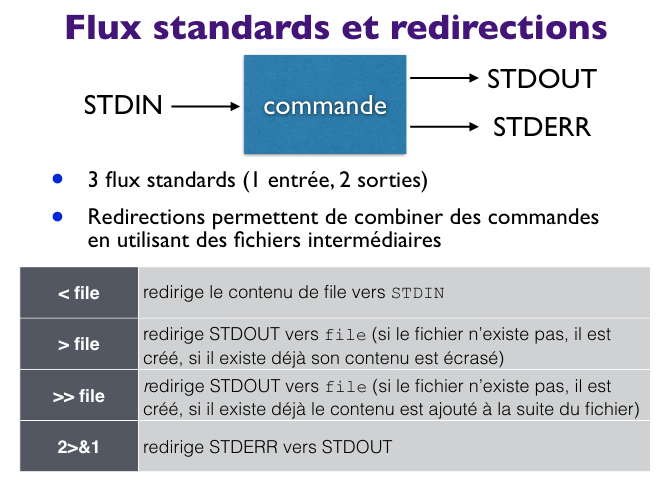
\includegraphics[scale=.5]{flux_std_et_redirections.png}\\
                Exemple de redirections :\\
                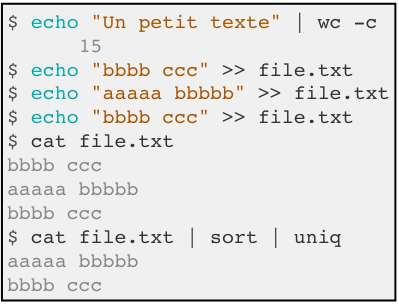
\includegraphics[scale=.5]{redirection_example.png}
            
                \subsubsection{Scripts}
                    Un système UNIX peut exécuter du language machine ou des \textbf{languages interprétés}
                    Un script commence par convention par les symboles $\#!$, référant à l'interpréteur, ici bin/bash :\\
                    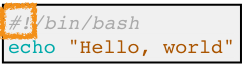
\includegraphics[scale=.7]{bash_script.png}\\\\
                    Ils peuvent aussi contenir des \textbf{variables}:\\
                    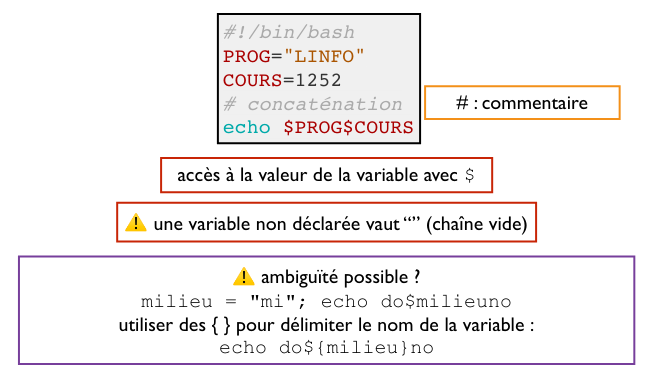
\includegraphics[scale=.5]{script_variables.png}\\\\
                    et des \textbf{conditionnelles} :\\
                    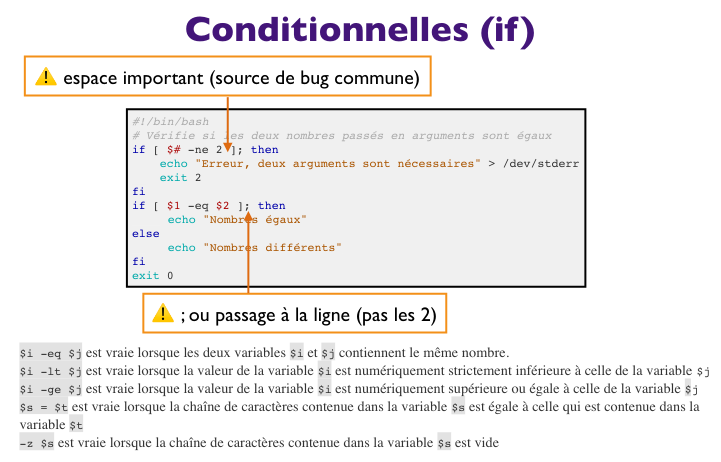
\includegraphics[scale=.5]{conditionnelles.png}\\
                    et des \textbf{boucles for}:\\
                    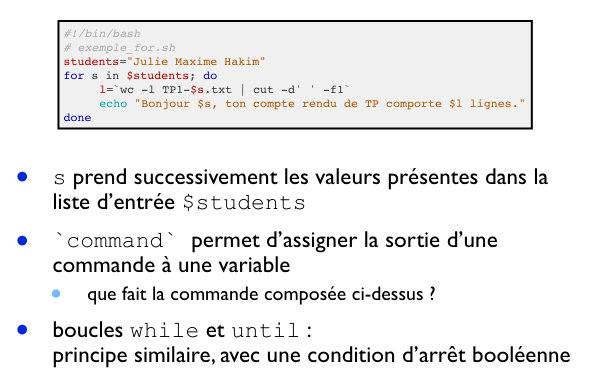
\includegraphics[scale=.6]{script_boucle_for.png}

    
\end{document}